\documentclass{article}
\usepackage{color}

\usepackage[utf8]{inputenc}
\usepackage[T1]{fontenc}
\usepackage[OT4,plmath]{polski}
\usepackage[pdftex]{color,graphicx}
\usepackage[a4paper,tmargin=3cm,bmargin=3cm,lmargin=3cm,rmargin=3cm]{geometry}
\usepackage{wrapfig}
\usepackage{amsmath}
\usepackage{amssymb}
\usepackage{lipsum}
\usepackage{tikz}
\usetikzlibrary{spath3, hobby, knots, braids, decorations, decorations.text}

\begin{document}
% \begin{tikzpicture}
%   \fill[white] (0,0) circle (.6);
%   \draw[line width=.8mm] (0,0) circle (.6);
%   \node at (.02,0) {$\color{gray}\boldsymbol{knmt}$};
%   \node at (0,0) {$\boldsymbol{knmt}$};
% \end{tikzpicture}
%
%
% \begin{tikzpicture}
%   \draw[line width=.8mm] (0,0) circle (.6);
%   \node at (.02,0) {$\color{gray}\boldsymbol{knmt}$};
%   \node at (0,0) {$\boldsymbol{knmt}$};
% \end{tikzpicture}


\fontsize{50}{45}\selectfont 
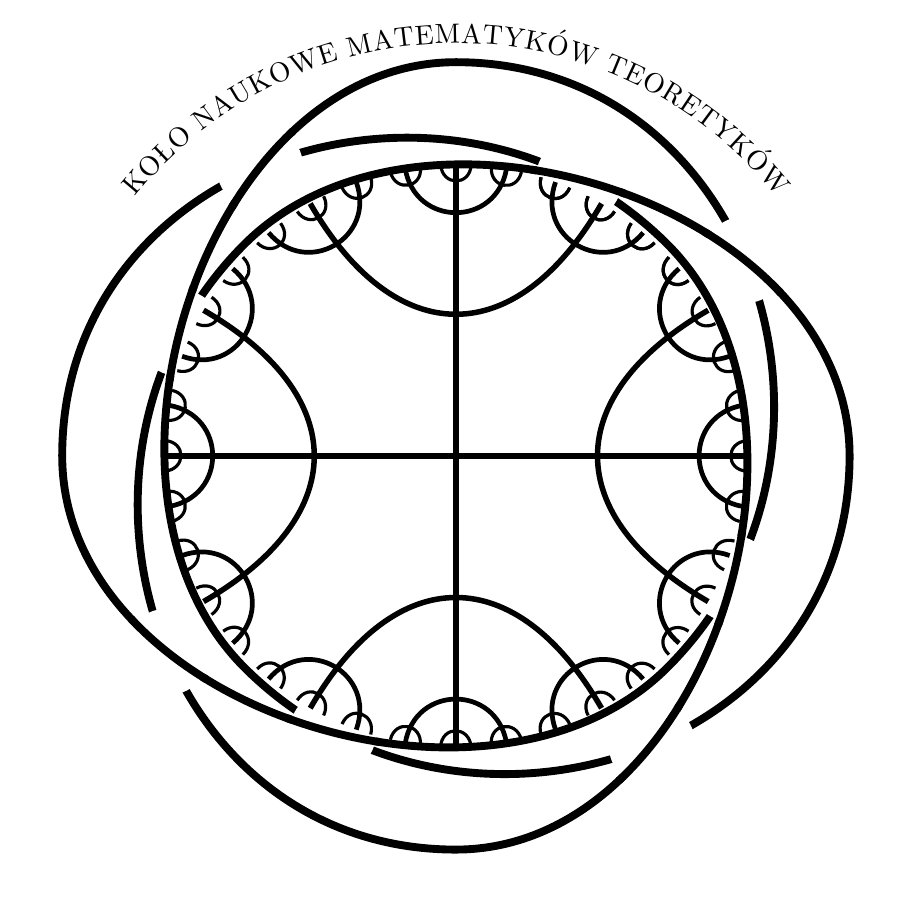
\begin{tikzpicture}
  \begin{scope}%[shift={(.25,0)}]%[rotate=15]
    \coordinate(n) at (90 :5);
    \coordinate(e) at (0  :5);
    \coordinate(s) at (-90:5);
    \coordinate(w) at (180:5);
    \coordinate(nw) at (135 :3.8);
    \coordinate(sw) at (-135:3.8);
    \coordinate(ne) at (45  :3.8);
    \coordinate(se) at (-45 :3.8);

    \begin{knot}[
      consider self intersections, 
      end tolerance=.01pt,
      clip width=20pt,
      clip radius=5.5mm,
      % draft mode=crossings,
      flip crossing=5,
      flip crossing=8,
      flip crossing=6,
      flip crossing=1,
      flip crossing=2,
      ]
      \strand[line width=1mm] (e)  to[out=-90, in=-45, looseness=1.2]
                     (sw) to[out=135, in=180]
                     (n)  to[out=0, in=45, looseness=1.2]
                     (se) to[out=-135, in=-90]
                     (w)  to[out=90, in=135, looseness=1.2]
                     (ne) to[out=-45, in=0]
                     (s)  to[out=180, in=-135, looseness=1.2]
                     (nw) to[out=45, in=90]
                     (e);
    \end{knot}
  \end{scope}

  \draw[line width=.7mm] (90:3.7)--(-90:3.7);
  \draw[line width=.7mm] (180:3.7)--(0:3.7);

  \foreach \i in {0, 1, 2, 3} {
    \draw[line width=.7mm] ({30+\i*90}:3.7) to[out={-150+\i*90}, in={150+\i*90}, looseness=1.5] ({-30+\i*90}:3.7);
  }

  \foreach \i in {0, 1, ..., 11} {
    \draw[line width=.6mm] ({40+\i*30}:3.7) to[out={-140+\i*30}, in={-160+\i*30}, looseness=1.5] ({20+\i*30}:3.7);
  }

  \foreach \i in {0, 1, ..., 39} {
    \draw[line width=.4mm] ({43+\i*10}:3.7) to[out={-135+\i*10}, in={-143+\i*10}, looseness=1.8] ({37+\i*10}:3.7);
  }

  \draw[color=white, rotate=-90, postaction={
                                    decorate, 
                                    decoration={
                                      text along path, 
                                      raise=4pt, 
                                      text align={align=center}, 
                                      text={ {KO{Ł}O NAUKOWE MATEMATYK{Ó}W TEORETYK{Ó}W} }, 
                                      reverse path
                                    }
                                  }] (0,0) circle (5.1);


\end{tikzpicture}

\end{document}
